\section{Introduction}
\label{sec:intro}
\vspace*{-3ex}
Programming languages such as Java and C++ provide exception-handling 
constructs such as \CodeIn{try-catch} to handle exception conditions that arise
during program execution. Under these exception conditions, programs follow paths
different from normal execution paths; these additional paths are referred to as 
\emph{exception} paths. Applications developed based on these programming
languages are expected to handle these exception conditions and take necessary recovery
actions. For example, when an application reuses resources such as files or database connections,
the application should release the resources after the usage in all paths
including \Intro{exception} paths. Failing to release the resources can not only cause performance degradation, 
but can also lead to critical issues. For example, if a database lock acquired by a
process is not released, any other process trying to acquire the same lock
hangs till the database releases the lock after timeout.
A case study~\cite{Weimer04} conducted on a real application 
demonstrates the necessity of releasing resources in exception paths 
for improving reliability and performance. 
The case study found that there was a surprising
improvement of 17\% in performance of the application after 
correctly releasing resources in the presence of exceptions.

\Comment{In general, software verification concentrates on verifying behaviors of the application 
during normal execution paths rather than exception paths. Therefore, the exception 
cases remain undetected during traditional software verification.}

Software verification can be challenging for exception cases as verification
techniques require specifications that describe expected behaviors when exceptions occur.
These specifications are often not available in practice~\cite{document:leth}.
To address this issue, association rules of the form ``$FC_a$ $\Rightarrow$ $FC_e$''
are mined as specifications~\cite{WeimerN05}, where both $FC_a$ and $FC_e$ are function calls that share
the same receiver object. These specifications are used to 
verify whether the function call $FC_a$ is followed by the function call $FC_e$ in all 
exception paths. However, simple association rules of this form are often not sufficient
to characterize common exception-handling rules. The rationale is that
there are various scenarios where $FC_a$ is not necessarily followed by $FC_e$ 
when exceptions are raised by $FC_a$, although both function calls 
share the same receiver object. 

\begin{figure*}[t]
\centering
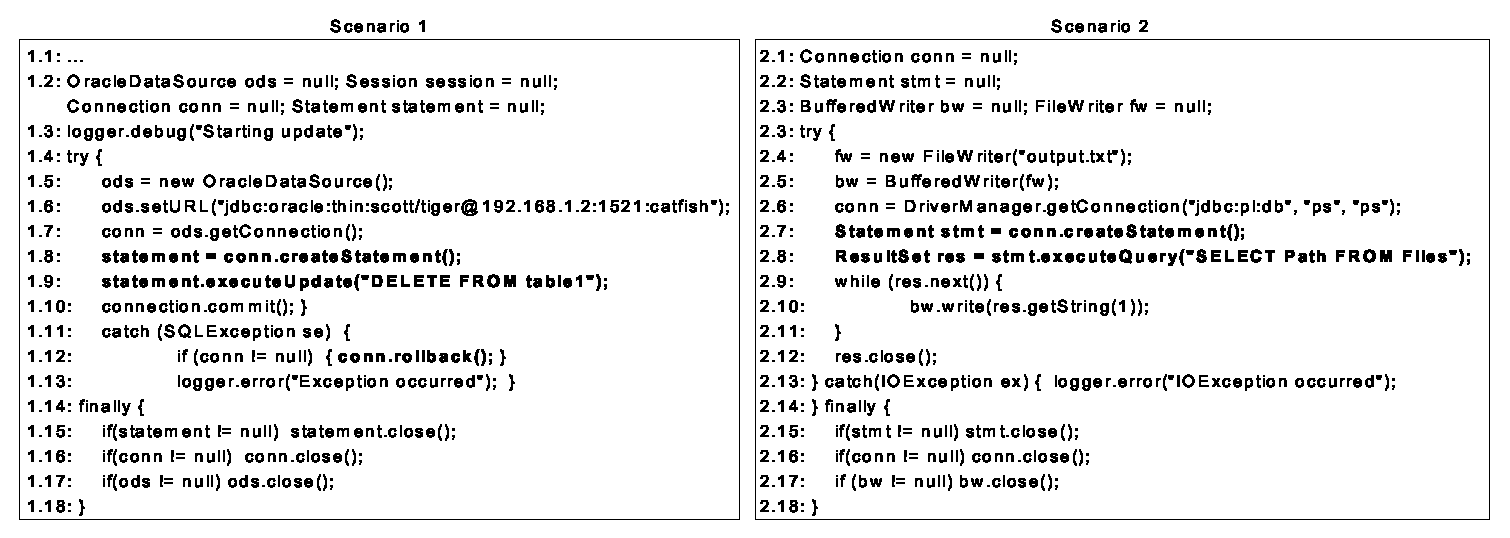
\includegraphics[scale=0.70,clip]{figs/three-code-examples1.eps}\vspace*{-3ex}
\centering \caption {\label{fig:threescenarios} Two example scenarios from real applications.}\vspace*{-4ex}
\end{figure*}

We next present an example using Scenarios 1 and 2 (extracted 
from real applications) shown in Figure~\ref{fig:threescenarios}. 
Scenario 1 attempts to modify contents of a database through the function call
\CodeIn{Statement.executeUpdate} (Line 1.9), whereas Scenario 2 attempts to read contents
of a database through the function call \CodeIn{Statement.executeQuery} (Line 2.8).
Consider a simple specification in the form of an association
rule ``\CodeIn{Connection creation} $\Rightarrow$
\CodeIn{Connection rollback}''. This rule describes that a \CodeIn{rollback} function call should
appear in exception paths whenever an object of \CodeIn{Connection} is created. 
Although a \CodeIn{Connection} object is created in both
scenarios, this rule applies only to Scenario 1 and does not apply to Scenario 2.
The primary reason is that the \CodeIn{rollback} function call should be invoked \emph{only} when 
there are any changes made to the database. This example shows that
simple association rules of the form ``$FC_a$ $\Rightarrow$ $FC_e$''
are often insufficient to characterize exception-handling rules.

The insufficiency of simple association rules calls for 
more general association rules, hereby referred to as \Intro{sequence association rules},
of the form ``($FC_c^1$...$FC_c^n$) $\wedge$ $FC_a$ $\Rightarrow$ ($FC_e^1$...$FC_e^m$)''.
This sequence association rule describes that function call $FC_a$ should be followed 
by function-call sequence $FC_e^1$...$FC_e^m$ in exception paths only 
when preceded by function-call sequence $FC_c^1$...$FC_c^n$. Using this sequence association rule,
the preceding example can be expressed as ``($FC_c^1$$FC_c^2$) $\wedge$ 
$FC_a$ $\Rightarrow$ ($FC_e^1$)'', where

$FC_c^1$ : \CodeIn{OracleDataSource.getConnection}\\
\hspace*{0.15in}$FC_c^2$ : \CodeIn{Connection.createStatement}\\
\hspace*{0.15in}$FC_a$ : \CodeIn{Statement.executeUpdate}\\
\hspace*{0.15in}$FC_e^1$ : \CodeIn{Connection.rollback}\\
\vspace*{-2ex}

This sequence association rule applies to Scenario 1 and
does not apply to Scenario 2 due to the presence of $FC_a$: \CodeIn{Statement.executeUpdate}.
The key aspects to be noted in this rule are: (1) \CodeIn{Statement.executeUpdate}
is the primary reason to have \CodeIn{Connection.rollback} in an exception path and
(2) the receiver object of \CodeIn{Statement.executeUpdate} is dependent on the 
receiver object of \CodeIn{Connection.rollback} through the function-call sequence
defined by $FC_c^1$$FC_c^2$.

Our sequence association rules are a super set of simple association rules.
For example, sequence association rules are the same as simple association
rules when the sequence $FC_c^1$...$FC_c^n$ is empty. 
To the best of our knowledge, existing association rule mining techniques~\cite{agarwal:association}
cannot be directly applied to mine these sequence association rules. 
Therefore, to bridge the gap, we develop a new mining algorithm by adapting the
frequent closed subsequence mining technique~\cite{wang:bide}. 

We further develop a novel approach, called CAR-Miner, that incorporates
our new mining algorithm for the problem of detecting exception-handling rules in
the form of sequence association rules by analyzing source code. Apart from mining sequence
association rules, CAR-Miner addresses another challenge that is often faced 
by existing approaches~\cite{Zhenmin2005PRMiner, chang07:finding, WeimerN05}, 
which mine rules from a limited data scope, 
i.e., from only a few example applications. Therefore, these approaches may not 
be able to mine rules that do not have enough
supporting samples in those example applications, and hence 
the related defects remain undetected by these approaches. To address
this challenge, CAR-Miner expands the data scope by leveraging a code search engine (CSE)
for gathering relevant code samples from existing open source projects available
on the web. From these relevant code samples, CAR-Miner mines exception-handling rules. 
We show the usefulness of mined exception-handling rules
by applying these rules on five applications to detect violations.
CAR-Miner tries to address problems related to the quality of code samples 
gathered from a CSE by capturing the most frequent patterns through mining.

\Comment{In particular, CAR-Miner accepts an input application and tries to detect
exception-handling defects in that application. Initially, CAR-Miner gathers function calls, referred as
$FC_a$, used by  the input application. CAR-Miner interacts with a code search engine (CSE) such as Google code search~\cite{GCSE} to gather related code examples that are already reusing $FC_a$. 
CAR-Miner constructs an Exception Flow Graph (EFG) for each code example gathered from 
the CSE. EFG is an extended form of control flow graph that captures flow of control in both
normal and exception conditions. While constructing EFG, we add only those exception
paths that can occur potentially during program execution. To capture such
exception paths, we use a sound static analysis that provides a set
of exceptions thrown by each $FC_a$ during program execution. 
CAR-Miner collects traces, which are
in the form of a sequence of function calls, from EFG post-processes these 
traces to filter unrelated function calls of $FC_a$.
CAR-Miner mines these traces to capture sequence association rules. 
Finally, CAR-Miner applies mined exception-handling rules to detect violations in the input application.
As CAR-Miner leverages a code search engine for gathering related code examples,
CAR-Miner has an added advantage of being able to mine rules, which do not have enough
supporting samples in the input application. CAR-Miner tries to address the 
problems related to the quality of the code examples 
gathered from a CSE by capturing the most frequent rule candidates through mining.}

This paper makes the following main contributions:\vspace*{-1ex}
\begin{Itemize}
\item A general mining algorithm to mine sequence association rules of the form 
``($FC_c^1$...$FC_c^n$) $\wedge$ $FC_a$ $\Rightarrow$ ($FC_e^1$...$FC_e^m$)''.
Our new mining algorithm takes a step forward in the direction 
of developing new mining algorithms to address
unique requirements in mining software engineering data, beyond being limited
by existing off-the-shelf mining algorithms.\vspace*{-2ex}
\item An approach that incorporates the general mining algorithm to mine exception-handling
rules that describe expected behavior when exceptions occur during
program execution. \vspace*{-2ex}
\item A technique for constructing a precise Exception-Flow Graph (EFG), which is an extended form of 
a Control-Flow Graph (CFG), that includes only those exception paths that can potentially occur 
during program execution.\vspace*{-2ex}
\item An implementation for expanding the data scope to open source projects that help
detect new related exception-handling rules that do not have enough supporting samples in an application under analysis.
These rules can help detect new defects in the application under analysis.\vspace*{-2ex}
\item Two evaluations to show
the effectiveness of our approach. (1) CAR-Miner detects $294$ real 
exception-handling rules in five different applications including $285$ KLOC. 
(2) The top $50$ exception-handling
rules (top $10$ real rules of each application)
are used to detect a total of $160$ real defects in these five
applications, where $87$ defects are new, not being detected by a 
previous related approach~\cite{WeimerN05}. \Comment{The initial response from 
developers of HsqlDB~\footnote{\url{http://hsqldb.sourceforge.net/}} is
encouraging. The developers responded on the first ten defects that we reported, 
where seven defects are \emph{accepted} and only three defects are rejected.}
\end{Itemize}

The rest of the paper is organized as follows. 
%Section~\ref{sec:example} presents example scenarios.
Section~\ref{sec:condrules} presents a formal definition of sequence
association rules and describes our new mining algorithm.
Section~\ref{sec:approach} describes key aspects of the CAR-Miner approach.
Section~\ref{sec:eval} presents evaluation results.
%Section~\ref{sec:discussion} presents limitations and future work.
Section~\ref{sec:threats} discusses threats to validity.
Section~\ref{sec:related} presents related work.
Finally, Section~\ref{sec:conclusion} concludes.

